\documentclass[12pt,a4paper]{article}

% ========== PACOTES ==========
\usepackage[utf8]{inputenc}
\usepackage[T1]{fontenc}
\usepackage[provide=*,portuguese]{babel}
\addto\captionsportuguese{\renewcommand{\figurename}{Figura}}
\addto\captionsportuguese{\renewcommand{\tablename}{Tabela}}
\usepackage{amsmath,amssymb,amsthm}
\usepackage{graphicx}
\usepackage[dvipsnames]{xcolor}
\usepackage{hyperref}
\usepackage{natbib}
\usepackage{geometry}
\usepackage{setspace}
\usepackage{enumitem}
\usepackage{booktabs}
\usepackage{longtable}
\usepackage{float}
\usepackage{caption}
\usepackage{footnote}
\usepackage{tcolorbox}
\usepackage{listings}
\usepackage{fancyhdr}
\usepackage{titlesec}
\usepackage{tocloft}
\usepackage{multicol}

\usepackage{tikz}
\usetikzlibrary{positioning,arrows.meta}

% ========== GEOMETRIA ==========
\geometry{a4paper, left=2.5cm, right=2.5cm, top=2.5cm, bottom=2.5cm}
\onehalfspacing

% ========== CORES ==========
\definecolor{clearblue}{RGB}{27,58,92}
\definecolor{clearlightblue}{RGB}{44,95,138}
\definecolor{salmonbg}{RGB}{252,235,230}
\definecolor{salmonframe}{RGB}{230,160,140}
\definecolor{bluebg}{RGB}{235,245,251}
\definecolor{blueframe}{RGB}{58,125,181}
\definecolor{orangebg}{RGB}{254,245,231}
\definecolor{orangeframe}{RGB}{230,126,34}
\definecolor{codebg}{RGB}{248,248,248}
\definecolor{codeframe}{RGB}{200,200,200}
\definecolor{Rblue}{RGB}{0,80,160}
\definecolor{Rgreen}{RGB}{0,128,0}
\definecolor{Rgray}{RGB}{128,128,128}

% ========== HYPERREF ==========
\hypersetup{
  colorlinks=true, linkcolor=clearlightblue, citecolor=clearlightblue, urlcolor=clearlightblue,
  pdfauthor={FGV CLEAR},
  pdftitle={Avaliação de Impacto: Pareamento (Matching)}
}

% ========== CABEÇALHOS ==========
\pagestyle{fancy}
\fancyhf{}
\fancyhead[R]{\small\textit{Guia CLEAR $|$ Pareamento (Matching)}}
\fancyfoot[C]{\thepage}
\renewcommand{\headrulewidth}{0pt}

% ========== TÍTULOS ==========
\titleformat{\section}{\Large\bfseries\color{clearblue}}{\thesection}{1em}{}
\titleformat{\subsection}{\large\bfseries\color{clearlightblue}}{\thesubsection}{1em}{}
\titleformat{\subsubsection}{\normalsize\bfseries\color{clearlightblue}}{\thesubsubsection}{1em}{}
\titleformat{\paragraph}[runin]{\normalsize\bfseries\itshape\color{clearblue}}{}{}{}[.]

% ========== CAIXAS ==========
\newtcolorbox{hipotesebox}[1][Hipóteses]{
  colback=salmonbg, colframe=salmonframe, coltitle=black, fonttitle=\bfseries,
  title=#1, boxrule=0.5pt, arc=2pt, left=6pt, right=6pt, top=4pt, bottom=4pt
}
\newtcolorbox{exemplobox}[1][Exemplo]{
  colback=salmonbg, colframe=salmonframe, coltitle=black, fonttitle=\bfseries,
  title=#1, boxrule=0.5pt, arc=2pt, left=6pt, right=6pt, top=4pt, bottom=4pt
}
\newtcolorbox{notabox}[1][Nota]{
  colback=bluebg, colframe=blueframe, coltitle=white, fonttitle=\bfseries,
  title=#1, boxrule=0.5pt, arc=2pt, left=6pt, right=6pt, top=4pt, bottom=4pt
}
\newtcolorbox{conexaobox}{
  colback=orangebg, colframe=orangeframe, boxrule=0.5pt, arc=2pt,
  left=6pt, right=6pt, top=3pt, bottom=3pt
}

% ========== LISTINGS ==========
\lstdefinestyle{Rstyle}{
  language=R, backgroundcolor=\color{codebg}, frame=single, rulecolor=\color{codeframe},
  basicstyle=\small\ttfamily, keywordstyle=\color{Rblue}\bfseries,
  stringstyle=\color{Rgreen}, commentstyle=\color{Rgray}\itshape,
  numbers=none, breaklines=true, showstringspaces=false, tabsize=2,
  xleftmargin=6pt, xrightmargin=6pt, aboveskip=8pt, belowskip=8pt,
  literate={á}{{\'a}}1 {é}{{\'e}}1 {í}{{\'i}}1 {ó}{{\'o}}1 {ú}{{\'u}}1
           {ã}{{\~a}}1 {õ}{{\~o}}1 {ç}{{\c{c}}}1 {ê}{{\^e}}1 {â}{{\^a}}1 {ô}{{\^o}}1
           {Á}{{\'A}}1 {É}{{\'E}}1 {Í}{{\'I}}1 {Ú}{{\'U}}1
           {<-}{{$\leftarrow$}}2
}
\lstdefinestyle{Routput}{
  backgroundcolor=\color{codebg}, frame=single, rulecolor=\color{codeframe},
  basicstyle=\small\ttfamily\color{Rgray}, numbers=none, breaklines=true,
  showstringspaces=false, xleftmargin=6pt, xrightmargin=6pt,
  aboveskip=4pt, belowskip=8pt
}

% ========== TEOREMAS ==========
\newtheorem{definicao}{Definição}[section]
\newtheorem{proposicao}{Proposição}[section]

% ========== METADADOS DE FIGURAS ==========
\newcommand{\figmeta}[3]{%
  \par\vspace{4pt}%
  \begin{minipage}{\linewidth}%
  \footnotesize%
  \textbf{Fonte:} #1\\%
  \textbf{Elaboração:} #2%
  \ifx&#3&\else\\[1pt]\textbf{Nota:} #3\fi%
  \end{minipage}%
  \vspace{6pt}%
}

% ========== DOCUMENTO ==========
\begin{document}

% ==========================================
% CAPA
% ==========================================
\thispagestyle{empty}
\begin{center}
\vspace*{4cm}
{\Large\bfseries\color{clearlightblue} SÉRIE: AVALIAÇÃO NA PRÁTICA}
\vspace{1.5cm}

{\Huge\bfseries\color{clearblue} Avaliação de Impacto:\\[0.3cm]
Pareamento\\[0.3cm]
(\textit{Matching})}

\vspace{2cm}
{\large FGV CLEAR $|$ FGV EESP $|$ Global Evaluation Initiative}

\vspace{0.5cm}
{\large [Mês/Ano]}

\vfill

\begin{abstract}
\noindent Este guia apresenta o método de pareamento (\textit{matching}) para avaliação de impacto de políticas públicas em dados observacionais. O pareamento constrói contrafactuais críveis ao aproximar as distribuições de covariáveis entre grupos tratados e de controle, operacionalizando a Hipótese de Independência Condicional. O guia cobre o arcabouço de resultados potenciais e o problema do viés de seleção, os métodos de pareamento exato e aproximado (vizinho mais próximo, \textit{kernel}), a distância de Mahalanobis, o \textit{propensity score} \citep{RosenbaumRubin1983}, a ponderação por probabilidade inversa (IPW) e notas sobre inferência. A replicação empírica utiliza os dados do \textit{National Supported Work Demonstration} \citep{LalondeNSW1986,DehejiaWahba1999} para ilustrar todas as etapas. Todos os exemplos incluem código completo em R.
\end{abstract}
\end{center}
\newpage

% ==========================================
% FICHA TÉCNICA
% ==========================================
\thispagestyle{empty}
\section*{Ficha Técnica}

\textbf{Organizadores:} [Nome 1], [Nome 2]

\textbf{Equipe técnica:} [Listar membros]

\vspace{1cm}

\noindent\textbf{Apresentação.} Este guia integra a série de publicações \textit{Avaliação na Prática}, desenvolvida pelo FGV CLEAR com o objetivo de ampliar o acesso a conhecimentos sobre monitoramento e avaliação com foco em políticas públicas.

Fundado em 2015, o FGV CLEAR tem se dedicado ao fortalecimento da cultura de gestão orientada por evidências no Brasil e em países lusófonos. Com sede na Escola de Economia de São Paulo da Fundação Getulio Vargas (FGV EESP), o FGV CLEAR atua como centro regional da Iniciativa CLEAR (\textit{Centers for Learning on Evaluation and Results}).

Saiba mais sobre o FGV CLEAR e acesse outras publicações em: \textbf{www.fgvclear.org}
\newpage

% ==========================================
% SUMÁRIO
% ==========================================
\tableofcontents
\newpage
% ==========================================
% SEÇÃO 1: INTRODUÇÃO
% ==========================================
\section{Introdução}\label{sec:introducao}

Em políticas públicas e avaliações de programas, um dos desafios centrais é estimar efetivamente qual o impacto de uma intervenção --- ou seja, distinguir o que mudou \textbf{por causa} da política do que teria mudado de qualquer forma. Para fazer isso com rigor, precisamos lidar com os chamados \textit{back-doors} no modelo causal: variáveis que influenciam tanto a participação na intervenção quanto o resultado e, assim, ameaçam a validade da comparação.

Num experimento, onde os grupos de tratamento e controle são aleatorizados, essas variáveis não seriam um problema para nossa comparação, já que a aleatorização da alocação do tratamento nos garantiria que as características dos dois grupos seriam iguais em média. No entanto, nem sempre conseguimos realizar sorteios, e selecionar todos os não-beneficiários de um programa como grupo de comparação provavelmente não resultará em uma comparação crível.

Considere o exemplo de um programa de qualificação profissional para jovens de baixa renda, como cursos de curta duração voltados para inserção no mercado de trabalho. Se compararmos diretamente a taxa de ocupação de participantes e não participantes, talvez encontremos que os primeiros têm maior empregabilidade após o curso. Mas esse resultado pode ser enganoso: é possível que os jovens que se inscreveram já fossem, em média, mais motivados, tivessem redes de contato melhores, ou nível educacional mais alto que os não inscritos. Nesse caso, a diferença observada não refletiria o efeito do programa, mas sim essas diferenças pré-existentes --- o chamado \textbf{viés de seleção}.

Esse problema é ubíquo em políticas públicas. Em saúde, por exemplo, indivíduos que aderem a campanhas de prevenção podem já ser mais conscientes sobre hábitos saudáveis; em educação, famílias que matriculam filhos em escolas de tempo integral podem diferir sistematicamente de outras em termos de renda ou engajamento.

Por isso, o desafio central da avaliação é criar comparações justas, isto é, contrafactuais\footnote{Contrafactuais representam os resultados potenciais que uma unidade teria apresentado caso estivesse submetida a uma condição diferente da observada. O efeito causal é definido como a diferença entre o resultado observado e o resultado contrafactual, este último não observável e estimado por métodos estatísticos \citep{ImbensRubin2015}.} que representem de forma plausível o que teria acontecido com os beneficiários caso não tivessem recebido o tratamento. Em termos operacionais, comparações justas exigem que unidades tratadas e não tratadas sejam comparáveis em todas as covariáveis relevantes que afetam simultaneamente a probabilidade de tratamento e o resultado, de modo que, condicional a essas características observáveis, a diferença média de resultados possa ser interpretada como efeito causal do programa.

O pareamento oferece uma resposta intuitiva a esse desafio: \textbf{para avaliar um programa, precisamos encontrar um grupo de comparação que se pareça o máximo possível com o grupo tratado}. Importante notar, contudo, que o pareamento não cria contrafactuais perfeitos, mas sim aproximações empíricas que são válidas sob hipóteses específicas sobre o processo de seleção. Em particular, o método procura simular uma situação experimental na qual tratados e controles são semelhantes em todas as características observáveis relevantes, diferenciando-se apenas pelo fato de terem (ou não) participado da política.

Voltando ao exemplo dos cursos de qualificação: em vez de comparar todos os inscritos com todos os não inscritos, podemos restringir a comparação apenas a jovens com perfis muito semelhantes --- por exemplo, mesma faixa etária, nível de escolaridade, gênero e bairro de residência. Essa estratégia, no entanto, só é viável quando existe \textbf{suporte comum} --- quando para cada perfil observado entre os participantes do curso há indivíduos comparáveis no grupo de não inscritos. Sob essa condição, se o curso teve impacto real, a diferença nos resultados de emprego entre esses grupos comparáveis será uma estimativa mais próxima do efeito verdadeiro.

A intuição é simples: ao eliminar diferenças observáveis entre tratados e controles, reduzimos o risco de atribuir ao programa algo que se deve, na verdade, a características pré-existentes dos participantes. É por isso que o \textit{pareamento} é frequentemente descrito como um método de \textbf{``construir contrafactuais''} usando dados observacionais. Essa estratégia, contudo, é suficiente apenas na medida em que as principais fontes de seleção no programa sejam observáveis e adequadamente controladas, hipótese conhecida como \textit{ignorabilidade} ou seleção em observáveis.

Essa abordagem é especialmente útil quando há um número razoável de variáveis observáveis que influenciam tanto a participação no tratamento quanto o desfecho de interesse, e quando há sobreposição entre os grupos. Assim, o pareamento se apresenta como uma ferramenta poderosa para estudos aplicados que buscam inferência causal em ambientes não experimentais.

O pareamento, apesar de ser uma ferramenta poderosa, requer cuidados na presença de viés de seleção associado a características observáveis, bem como na escolha de métricas de distância e na avaliação da qualidade do balanceamento entre tratados e controles. Por outro lado, vieses decorrentes de fatores não observáveis que afetam simultaneamente a participação no programa e os resultados não são, em geral, corrigíveis por pareamento. Portanto, também discutiremos técnicas de diagnóstico e procedimentos de avaliação da qualidade do pareamento, conforme sugerido por \citet{abadie2006large} e \citet{imbens2004nonparametric}.

O restante do guia está organizado da seguinte forma. A Seção~\ref{sec:causalidade} apresenta o arcabouço causal, introduzindo o modelo de resultados potenciais, o problema do viés de seleção e a distinção entre dados experimentais e não-experimentais, utilizando um programa real como exemplo motivador. A Seção~\ref{sec:pareamento} introduz o método de pareamento, discutindo sua lógica de identificação e sua relação com a construção de contrafactuais em dados observacionais. As Seções~\ref{sec:univariado} e~\ref{sec:multivariado} detalham os principais métodos operacionais, começando pelo caso univariado e avançando para o pareamento com múltiplas covariáveis, incluindo o uso do \textit{propensity score}. A Seção~\ref{sec:diagnosticos} discute extensões, diagnósticos e armadilhas comuns. A Seção~\ref{sec:aplicacoes} apresenta aplicações em políticas públicas. Por fim, a Seção~\ref{sec:conclusao} conclui com limitações e conexões com outros métodos.

% ==========================================
% SEÇÃO 2: CAUSALIDADE
% ==========================================
\newpage
\section{Causalidade e o Problema do Contrafactual}\label{sec:causalidade}

Antes de introduzirmos o pareamento, é necessário discutir a causalidade de maneira mais formal. Esta seção tem como objetivo fixar a notação básica, definir os principais estimandos de interesse e explicitar o problema do viés de seleção que surge na ausência de um desenho experimental. Para tanto, utilizaremos um exemplo real de política de treinamento que acompanhará o restante do guia.

\subsection{Avaliando um Programa de Treinamento}

O \textit{National Supported Work Demonstration} (NSW) foi um programa de treinamento profissional conduzido nos Estados Unidos na metade da década de 1970 pela \textit{Manpower Demonstration Research Corporation} (MDRC). O objetivo principal do NSW era ajudar trabalhadores em situação de vulnerabilidade, que tinham pouca experiência ou qualificações, a se inserir no mercado de trabalho. O programa oferecia emprego temporário, treinamento e acompanhamento psicológico dentro de um ambiente protegido.

Os participantes selecionados recebiam emprego garantido por 9 a 18 meses. Trabalhavam em equipes pequenas e se reuniam regularmente com um conselheiro do programa para discutir dificuldades e desempenho. O trabalho era remunerado, embora com salários inferiores aos de empregos regulares, mas havia possibilidade de aumento conforme o desempenho e a assiduidade. Após o término do contrato, os participantes precisavam buscar trabalho no mercado comum.

Para avaliar o impacto do programa, a MDRC coletou dados sobre renda e características demográficas dos participantes e do grupo de controle no período inicial e em até quatro entrevistas de acompanhamento realizadas a cada nove meses. Esses dados serviram para medir como o programa influenciava o emprego e a renda ao longo do tempo, sendo um dos primeiros experimentos sociais randomizados em políticas de emprego e uma referência clássica em avaliação de impacto \citep{LalondeNSW1986}.

Ao longo desse guia, utilizaremos o \textit{software} R para manipular os dados e estimar os resultados. Vamos começar limpando o ambiente e carregando os pacotes necessários.

\begin{lstlisting}[style=Rstyle]
# Limpar o ambiente
rm(list = ls())

library(tidyverse)   # Manipulação de dados + gráficos
library(haven)       # Abre diversos tipos de arquivos

# Estimação
library(sandwich)
library(lmtest)
library(estimatr)

# Visualização
library(modelsummary)
library(kableExtra)
\end{lstlisting}

Para baixarmos os dados, criamos uma função que acessa o repositório público:

\begin{lstlisting}[style=Rstyle]
baixar_dados <- function(dados) {
  link <- paste("https://github.com/scunning1975/mixtape/raw/master/",
                dados, sep = "")
  df <- read_dta(link)
  return(df)
}

nsw <- baixar_dados("nsw_mixtape.dta")
\end{lstlisting}

Por fim, criaremos algumas variáveis que serão utilizadas nas análises:

\begin{lstlisting}[style=Rstyle]
nsw <- nsw %>%
  mutate(
    agesq    = age^2,          # Idade ao quadrado
    agecube  = age^3,          # Idade ao cubo
    educsq   = educ^2,         # Educação ao quadrado
    u74      = case_when(re74 == 0 ~ 1, TRUE ~ 0),  # Desemprego 1974
    u75      = case_when(re75 == 0 ~ 1, TRUE ~ 0),  # Desemprego 1975
    re74sq   = re74^2,         # Renda 1974 ao quadrado
    re75sq   = re75^2          # Renda 1975 ao quadrado
  )
\end{lstlisting}

\subsection{Resultados Potenciais}\label{sec:po}

A avaliação do programa NSW tem como objetivo principal estimar os efeitos da participação sobre os ganhos monetários reais dos participantes. Seguindo a lógica de \citet{ImbensRubin2015}, para cada indivíduo $i = 1,\dots,N$, definimos os resultados potenciais:

\begin{itemize}
    \item $Y_i(1)$ é o ganho monetário real do indivíduo $i$ caso ele participe do programa;
    \item $Y_i(0)$ é o ganho monetário real do indivíduo $i$ caso ele \textbf{não} participe do programa.
\end{itemize}

Assim, é possível definir o efeito causal do programa NSW \textbf{para cada indivíduo $i$}:
$$\delta_i = Y_i(1) - Y_i(0)$$

Esse parâmetro captura a diferença entre os ganhos monetários reais que um indivíduo teria caso participasse do programa e aqueles que teria caso não participasse. No entanto, para cada indivíduo, apenas um desses resultados potenciais é observado em um dado período. Seja $D_i = 1$ caso o indivíduo $i$ tenha participado do programa e $D_i = 0$ caso contrário, o resultado observado pode ser escrito como:
$$Y_i = D_i Y_i(1) + (1 - D_i) Y_i(0)$$

Como não é possível comparar os dois resultados potenciais de um mesmo indivíduo, tentaremos comparar indivíduos que participaram com aqueles que não participaram. Nosso objetivo é estimar o Efeito Médio do Tratamento (\textit{Average Treatment Effect} --- ATE) ou o Efeito Médio do Tratamento nos Tratados (\textit{Average Treatment Effect on the Treated} --- ATT), definidos por:
$$\text{ATE} = \mathbb{E}[Y_i(1) - Y_i(0)], \qquad \text{ATT} = \mathbb{E}[Y_i(1) - Y_i(0) \mid D_i = 1]$$

\textbf{Será que conseguimos recuperar o ATE ou o ATT apenas comparando a média dos grupos?} A comparação simples de médias pode ser decomposta como:

\begin{equation}\label{eq:viesselecao}
    \begin{split}
        \mathbb{E}[Y_i \mid D_i = 1] - \mathbb{E}[Y_i \mid D_i = 0]
        &= \underbrace{\mathbb{E}[Y_i(1) \mid D_i = 1] - \mathbb{E}[Y_i(0) \mid D_i = 1]}_{\text{ATT}} \\
        &+ \underbrace{\mathbb{E}[Y_i(0) \mid D_i = 1] - \mathbb{E}[Y_i(0) \mid D_i = 0]}_{\text{Viés de Seleção}}
    \end{split}
\end{equation}

A Equação~\eqref{eq:viesselecao} mostra que a simples comparação de médias estará potencialmente viesada. O viés de seleção reflete a presença de características individuais que influenciam simultaneamente a decisão de participar do programa e os ganhos monetários potenciais. Imagine, por exemplo, que a divulgação do programa NSW tenha atingido majoritariamente pessoas de maior escolaridade. Podemos visualizar as direções da causalidade no grafo abaixo:

\[
\begin{array}{ccccc}
  & & \text{Escolaridade} & & \\
  & \swarrow & & \searrow \\
  D & &\longrightarrow && Y
\end{array}
\]

Neste caso, ao compararmos os grupos, estamos essencialmente comparando os ganhos de pessoas com maior escolaridade com ganhos de pessoas com menor escolaridade, o que introduz viés de seleção.

\subsection{Experimentos Aleatorizados}

O diferencial do NSW é que ele foi um experimento aleatorizado: entre os candidatos elegíveis, alguns foram escolhidos aleatoriamente para participar, enquanto outros não foram selecionados e serviram como grupo de controle.

A aleatorização nos garante que a alocação do tratamento não depende de nenhuma característica individual. Em termos matemáticos:
$$(Y_i(1), Y_i(0)) \perp D_i$$

ou seja, participar ou não do programa é independente dos ganhos monetários potenciais. Em um experimento aleatorizado, podemos verificar empiricamente se os grupos de tratamento e controle são semelhantes em termos das características \textbf{observáveis} $X_i$ --- esse procedimento é conhecido como \textbf{análise de balanceamento}. No R, utilizaremos o pacote \texttt{vtable}:

\begin{lstlisting}[style=Rstyle]
library(vtable)

nsw %>%
  select(c("treat", "age", "educ", "nodegree", "marr",
           "black", "hisp", "re74", "re75", "u74", "u75")) %>%
  sumtable(group = "treat", group.test = TRUE, digits = 3)
\end{lstlisting}

\begin{table}[H]
\centering
\caption{Balanceamento --- Experimento NSW}\label{tab:balance}
\begin{tabular}{lccccccl}
\toprule
Tratamento & \multicolumn{3}{c}{0} & \multicolumn{3}{c}{1} & \\
\midrule
Variável & N & Média & DP & N & Média & DP & Teste F \\
\midrule
Idade              & 260 & 25,1  & 7,06 & 185 & 25,8  & 7,16 & $F=1{,}247$      \\
Educação           & 260 & 10,1  & 1,61 & 185 & 10,3  & 2,01 & $F=2{,}237$      \\
E.M. Incompleto    & 260 & 0,835 & 0,372 & 185 & 0,708 & 0,456 & $F=10{,}338^{***}$ \\
Pardo              & 260 & 0,154 & 0,361 & 185 & 0,189 & 0,393 & $F=0{,}961$      \\
Negro              & 260 & 0,827 & 0,379 & 185 & 0,843 & 0,365 & $F=0{,}207$      \\
Hispânico          & 260 & 0,108 & 0,311 & 185 & 0,060 & 0,237 & $F=3{,}153^{*}$  \\
Renda 1974         & 260 & 2.107 & 5.688 & 185 & 2.096 & 4.887 & $F=0{,}000$      \\
Renda 1975         & 260 & 1.267 & 3.103 & 185 & 1.532 & 3.219 & $F=0{,}765$      \\
Desemprego 1974    & 260 & 0,750 & 0,434 & 185 & 0,708 & 0,456 & $F=0{,}966$      \\
Desemprego 1975    & 260 & 0,685 & 0,466 & 185 & 0,600 & 0,491 & $F=3{,}410^{*}$  \\
\midrule
\multicolumn{8}{l}{\footnotesize Significância estatística: $^{*}\,p<0{,}1$;\; $^{**}\,p<0{,}05$;\; $^{***}\,p<0{,}01$}\\
\end{tabular}
\end{table}

O ponto central da Tabela~\ref{tab:balance} é gerar evidência de que a alocação do tratamento não está correlacionada com nenhuma característica observada. Um bom balanceamento adicionado à aleatorização garantem que o viés de seleção deixe de existir, e a comparação de médias é igual ao ATT:
$$\mathbb{E}[Y_i \mid D_i = 1] - \mathbb{E}[Y_i \mid D_i = 0] = \mathbb{E}[Y_i(1) \mid D_i = 1] - \mathbb{E}[Y_i(0) \mid D_i = 1] = \text{ATT}$$

Podemos estimar o efeito causal via regressão simples:

\begin{lstlisting}[style=Rstyle]
# Igual à diferença de médias
fit_nsw <- lm_robust(re78 ~ treat, se_type = "stata", data = nsw)
summary(fit_nsw)
\end{lstlisting}

\begin{table}[H]
\centering
\caption{Resultado da Regressão --- Dados Experimentais}\label{tab:reg1}
\begin{tabular}{lc}
\toprule
 & Estimativa \\
\midrule
Intercepto \hspace{60mm} & 4.554,801*** \\
 & (340,204) \\
Tratamento & 1.794,342** \\
 & (670,824) \\
Observações & 445 \\
\bottomrule
\multicolumn{2}{l}{\footnotesize $^{+}\,p<0{,}1$;\; $^{*}\,p<0{,}05$;\; $^{**}\,p<0{,}01$;\; $^{***}\,p<0{,}001$}\\
\end{tabular}
\end{table}

A Tabela~\ref{tab:reg1} indica que o programa NSW \textbf{causou}, em média, um aumento de \$1.794,34 aos participantes do programa.

\subsection{Dados Não-Experimentais}

Até aqui, utilizamos o programa NSW como um exemplo ideal de avaliação causal. No entanto, esse tipo de desenho é a exceção, e não a regra, na avaliação de políticas públicas. Na grande maioria das situações, o pesquisador dispõe apenas de dados observacionais, gerados sem qualquer controle direto sobre o processo de seleção para o tratamento.

Para ilustrar esse cenário, vamos considerar a \textit{Current Population Survey} (CPS), uma pesquisa domiciliar representativa da população dos Estados Unidos. Ao compararmos os participantes do NSW com indivíduos da CPS como controle, estamos comparando grupos que podem ser estruturalmente muito diferentes entre si:

\begin{lstlisting}[style=Rstyle]
# Baixar dados não-experimentais
cps <- baixar_dados("cps_mixtape.dta")

# Juntar com o grupo tratado do NSW
nsw_treat <- nsw %>% filter(treat == 1)

cps <- cps %>%
  bind_rows(nsw_treat) %>%
  mutate(
    agesq   = age^2,
    agecube = age^3,
    educsq  = educ * educ,
    u74     = case_when(re74 == 0 ~ 1, TRUE ~ 0),
    u75     = case_when(re75 == 0 ~ 1, TRUE ~ 0),
    re74sq  = re74^2,
    re75sq  = re75^2
  )

# Diferença simples entre tratados e controle não-experimental
fit_nswcps <- lm_robust(re78 ~ treat, se_type = "stata", data = cps)
summary(fit_nswcps)
\end{lstlisting}

\begin{table}[H]
\centering
\caption{Resultado da Regressão --- Dados Não-Experimentais}\label{tab:reg2}
\begin{tabular}{lc}
\toprule
 & Estimativa \\
\midrule
Intercepto \hspace{60mm} & 14.846,660*** \\
 & (76,291) \\
Tratamento & $-$8.497,516*** \\
 & (581,916) \\
Observações & 16.177 \\
\bottomrule
\multicolumn{2}{l}{\footnotesize $^{+}\,p<0{,}1$;\; $^{*}\,p<0{,}05$;\; $^{**}\,p<0{,}01$;\; $^{***}\,p<0{,}001$}\\
\end{tabular}
\end{table}

O contraste entre as Tabelas~\ref{tab:reg1} e~\ref{tab:reg2} é revelador. Enquanto a regressão com dados experimentais aponta um efeito positivo e significativo do tratamento, a regressão com dados não experimentais produz uma estimativa fortemente negativa. Essa reversão de sinal não decorre de um efeito causal adverso do programa, mas sim de viés de seleção: participantes do programa têm, em média, piores condições iniciais no mercado de trabalho do que a população geral da CPS.

\subsection{Ajustando pelas Características Observáveis}

Uma resposta natural ao problema é tentar ``corrigir'' a comparação ajustando pelas características observáveis dos indivíduos. Em vez da regressão simples, passamos a estimar:
\begin{equation}\label{eq:olscov}
    Y_i = \alpha + \beta D_i + X_i'\gamma + \varepsilon_i
\end{equation}

em que $X_i$ é um vetor de características observáveis. Podemos também utilizar a regressão de Lin \citep{LinRegression2013}, que adiciona interações entre o tratamento e cada uma das covariáveis:
\begin{equation}\label{eq:olslin}
    Y_i = \alpha + \beta D_i + X_i' \gamma + (D_i \cdot X_i)' \delta + \varepsilon_i
\end{equation}

\begin{lstlisting}[style=Rstyle]
# Ajustando por covariáveis (NSW)
fit_nsw_cov <- lm_robust(re78 ~ treat + age + agesq + educ + nodegree +
                           marr + black + hisp + re74 + re75 + u74 + u75,
                         se_type = "stata", data = nsw)

# Regressão de Lin (NSW)
fit_nsw_lin <- lm_lin(re78 ~ treat,
                      covariates = ~ age + agesq + educ + nodegree +
                                    marr + black + hisp + re74 + re75 + u74 + u75,
                      se_type = "stata", data = nsw)

# Ajustando por covariáveis (NSW + CPS)
fit_nswcps_cov <- lm_robust(re78 ~ treat + age + agesq + educ + nodegree +
                              marr + black + hisp + re74 + re75 + u74 + u75,
                            se_type = "stata", data = cps)

# Regressão de Lin (NSW + CPS)
fit_nswcps_lin <- lm_lin(re78 ~ treat,
                         covariates = ~ age + agesq + educ + nodegree +
                                       marr + black + hisp + re74 + re75 + u74 + u75,
                         se_type = "stata", data = cps)
\end{lstlisting}

\begin{table}[H]
\centering
\caption{Regressões ajustadas com dados experimentais e não-experimentais}\label{tab:reg3}
\begin{tabular}{lcc}
\toprule
 & Coef.\ Tratamento & Obs. \\
\midrule
NSW --- Sem covariáveis                & 1.794,342** & 445 \\
                                       & (670,824) & \\
NSW --- Com covariáveis                & 1.669,843* & 445 \\
                                       & (680,269) & \\
NSW --- Covariáveis (Lin) \hspace{20mm}& 1.567,145* & 445 \\
                                       & (662,403) & \\
NSW+CPS --- Sem covariáveis            & $-$8.497,516*** & 16.177 \\
                                       & (581,916) & \\
NSW+CPS --- Com covariáveis            & 1.137,196$^+$ & 16.177 \\
                                       & (627,993) & \\
NSW+CPS --- Covariáveis (Lin)          & $-$5.149,338 & 16.177 \\
                                       & (3.255,997) & \\
\bottomrule
\multicolumn{3}{l}{\footnotesize $^{+}\,p<0{,}1$;\; $^{*}\,p<0{,}05$;\; $^{**}\,p<0{,}01$;\; $^{***}\,p<0{,}001$}\\
\end{tabular}
\end{table}

A Tabela~\ref{tab:reg3} evidencia que, na amostra experimental do NSW, a estimativa permanece positiva e significativa após o controle por covariáveis. Em contraste, quando a amostra não-experimental da CPS é incorporada, as estimativas mudam drasticamente, indicando que o simples controle linear é insuficiente para eliminar o viés de seleção.

No entanto, a regressão múltipla ainda não garante identificação causal. Para que o coeficiente $\beta$ possa ser interpretado causalmente, é necessário assumir a \textbf{Hipótese de Independência Condicional}:

\begin{hipotesebox}[Hipótese de Independência Condicional (CIA)]
Condicionalmente ao vetor de covariáveis $X_i$, a participação no programa é independente dos resultados potenciais:
$$(Y_i(1), Y_i(0)) \perp D_i \mid X_i$$
Adicionalmente, é necessária a condição de \textbf{suporte comum}: para todo $x$ no suporte dos tratados, $0 < \mathbb{P}(D_i = 1 \mid X_i = x) < 1$.
\end{hipotesebox}

Essa condição afirma que, após o controle por um conjunto suficiente de covariáveis, não restariam fatores não observados que afetassem simultaneamente a decisão de participar do programa e o resultado. A regressão apresenta, no entanto, limitações centrais: (i) ela é uma suposição forte e não testável; (ii) depende de forma funcional específica; e (iii) pode sofrer com falta de sobreposição e extrapolação. É exatamente nesse ponto que entra o \textit{pareamento}, discutido na próxima seção.

\begin{notabox}[Quais covariáveis incluir? O papel dos DAGs]
A escolha do conjunto de covariáveis $X_i$ é a decisão mais importante de toda a análise de pareamento --- e também a mais sujeita a erros silenciosos. A CIA é não testável; sua plausibilidade depende inteiramente de incluir as variáveis certas.

\textbf{Variáveis que devem entrar:} todas as características observadas que influenciam simultaneamente a probabilidade de tratamento \textit{e} o resultado de interesse. No exemplo do NSW: renda anterior (\texttt{re74}, \texttt{re75}), escolaridade, raça, situação no mercado de trabalho pré-intervenção.

\textbf{Três erros comuns a evitar:}
\begin{enumerate}[leftmargin=1.5em, itemsep=2pt]
  \item \textbf{Variáveis pós-tratamento}: incluir variáveis que podem ser afetadas pelo tratamento (ex.: renda de 1978 como covariável para estimar o efeito do tratamento de 1977) introduz viés de mediação, não o elimina.
  \item \textbf{\textit{Colliders}}: variáveis que são causadas simultaneamente pelo tratamento e pelo resultado. Condicionar em um \textit{collider} reabre um caminho de viés que estava bloqueado.
  \item \textbf{Variáveis irrelevantes}: incluir muitas covariáveis sem relação com o tratamento prejudica o suporte comum e eleva a variância do estimador, sem ganho identificatório.
\end{enumerate}

\textbf{Ferramenta recomendada:} construa um Grafo Acíclico Dirigido (DAG) da estrutura causal do problema antes de definir $X_i$. O DAG torna explícitas as hipóteses sobre o processo de geração dos dados e permite identificar quais variáveis são confundidoras legítimas, quais são \textit{colliders} e quais são mediadores. O pacote \texttt{dagitty} no R facilita esse exercício.
\end{notabox}

% ==========================================
% SEÇÃO 3: O MÉTODO DE PAREAMENTO
% ==========================================
\newpage
\section{O Método de Pareamento}\label{sec:pareamento}

Na seção anterior, vimos que, para identificar um efeito causal em dados não-experimentais, precisamos comparar o que de fato ocorreu com o que teria acontecido na ausência da política. A regressão é a ferramenta mais usada para esse propósito, mas sua validade causal depende de hipóteses fortes. Por esse motivo, é útil considerar estratégias alternativas para lidar com o viés de seleção.

O pareamento nasce exatamente desse incômodo. Em vez de depender de uma forma funcional ou de um ajuste paramétrico, ele parte de uma ideia mais direta: \textbf{se quisermos saber o que teria acontecido com os tratados, comparemos com não tratados que se pareçam com eles}. A lógica é simples, mas poderosa. Se cada beneficiário do programa tiver uma ``dupla'' no grupo de controle com características muito próximas, então a diferença média entre os dois grupos fornece uma boa aproximação do efeito causal.

A diferença central em relação à regressão está na ordem lógica do procedimento. No pareamento, a comparabilidade entre tratados e controles é construída primeiro, por meio da restrição explícita do conjunto de comparação; a estimação do efeito vem depois, como uma simples diferença de médias. O avaliador não está modelando a relação entre variáveis, e sim \textbf{selecionando comparações justas}.

\subsection{A Ideia Central do Pareamento}

A CIA garante que, dentro de cada célula $X_i = x$, a seleção no tratamento é ``como se fosse aleatória''. Com isso, o efeito causal local é identificado diretamente pela diferença de médias observada:
\[
\delta(x)
=
\mathbb{E}[Y_i \mid D_i = 1, X_i = x]
-
\mathbb{E}[Y_i \mid D_i = 0, X_i = x]
=
\text{ATE}(x)
=
\text{ATT}(x)
\]

Uma vez identificados os efeitos causais locais $\delta(x)$, os parâmetros agregados surgem como médias ponderadas:
\[
\text{ATE}
=
\sum_x \delta(x)\,\mathbb{P}(X_i = x),
\qquad
\text{ATT}
=
\sum_x \delta(x)\,\mathbb{P}(X_i = x \mid D_i = 1)
\]

Se o vetor $X_i$ fosse simples, essa estimação seria direta. Com apenas uma covariável, bastaria calcular a diferença de médias condicional. Na maior parte das aplicações empíricas, contudo, o vetor $X_i$ é substancialmente mais complexo. O espaço de covariáveis se torna rapidamente esparso à medida que a dimensão aumenta --- a chamada \textit{maldição da dimensionalidade}. É exatamente nesse ponto que o pareamento se torna útil.

\subsection{Pareamento Exato}

O pareamento exato representa a forma mais direta de tornar tratados e controles comparáveis. Para cada indivíduo tratado, buscamos no grupo de controle apenas indivíduos que tenham exatamente os mesmos valores em todas as covariáveis utilizadas.

Considere um exemplo com duas covariáveis --- escolaridade e experiência prévia --- e três tratados:

\begin{table}[H]
\centering
\caption{Amostra hipotética para pareamento exato}\label{tab:exato1}
\begin{tabular}{lllll}
\toprule
Indivíduo & Tratamento & Escolaridade & Exp.\ prévia & Salário \\
\midrule
A & 1 & Baixa & Não & 1.200 \\
B & 1 & Alta  & Não & 1.400 \\
C & 1 & Baixa & Sim & 1.300 \\
1 & 0 & Baixa & Não & 900   \\
2 & 0 & Alta  & Não & 1.050 \\
3 & 0 & Baixa & Sim & 1.000 \\
4 & 0 & Alta  & Sim & 1.150 \\
\bottomrule
\end{tabular}
\end{table}

Aplicando o pareamento exato, cada tratado é comparado com o controle de perfil idêntico:

\begin{table}[H]
\centering
\caption{Efeitos individuais no pareamento exato}\label{tab:exato2}
\begin{tabular}{llll}
\toprule
Tratado & Salário tratado & Salário controle & Efeito \\
\midrule
A & 1.200 & 900   & 300 \\
B & 1.400 & 1.050 & 350 \\
C & 1.300 & 1.000 & 300 \\
\bottomrule
\end{tabular}
\end{table}

O ATT estimado é $\widehat{\text{ATT}} = (300 + 350 + 300)/3 = 316{,}7$. O controle~4 não é utilizado pois não existe nenhum tratado com escolaridade alta e experiência prévia simultaneamente.

Essa força é também a principal limitação do método. À medida que o número de covariáveis cresce, o espaço de combinações explode e muitos estratos passam a conter apenas tratados ou apenas controles --- tornando o pareamento exato inviável na prática com muitas variáveis.

\subsection{Pareamento como Médias Ponderadas}

Quando não existe ninguém no grupo de controle exatamente igual a um tratado, passamos a usar vários controles ``parecidos'', combinados por meio de uma média ponderada. Essa transição não relaxa a hipótese de independência condicional --- o que se relaxa é apenas a exigência operacional de igualdade exata.

A lógica pode ser escrita como:
$$\tilde{Y}_i = \sum_{j \in \mathcal{C}} w_{ij} Y_j$$

em que $\mathcal{C}$ é o conjunto de controles e os pesos $w_{ij}$ somam 1. A diferença entre os métodos de pareamento está exatamente na forma como esses pesos são definidos:

\begin{itemize}
  \item No \textbf{pareamento exato}, apenas os controles idênticos ao tratado recebem peso (igual);
  \item No \textbf{vizinho mais próximo}, apenas o(s) controle(s) mais próximo(s) recebem peso;
  \item No \textbf{pareamento por \textit{kernel}}, todos os controles recebem peso, que decai continuamente com a distância.
\end{itemize}

Essa interpretação como médias ponderadas também esclarece a relação entre pareamento e regressão: na regressão, a ponderação é implícita e determinada pela forma funcional; no pareamento, ela é construída explicitamente com base na similaridade entre indivíduos.

% ==========================================
% SEÇÃO 4: PAREAMENTO COM UMA VARIÁVEL
% ==========================================
\newpage
\section{Pareamento com Uma Variável}\label{sec:univariado}

Para entender como o pareamento funciona na prática, é útil começar pelo caso mais simples possível: o pareamento baseado em uma única variável. Esse exercício é didaticamente poderoso porque todas as decisões fundamentais do pareamento já aparecem de forma clara, sem a complexidade adicional trazida por múltiplas covariáveis.

Suponha, no contexto do NSW, que decidimos comparar tratados e controles apenas com base na escolaridade. Mesmo nesse caso unidimensional, somos obrigados a responder uma sequência de decisões fundamentais:

\begin{enumerate}
  \item \textbf{Critério de pareamento:} qual será nossa noção de ``semelhança''? Dois indivíduos com 10 e 11 anos de estudo são comparáveis? E 10 e 12?
  \item \textbf{Selecionar pares ou ponderar?} Para cada tratado, escolhemos controles específicos ou construímos uma amostra ponderada?
  \item \textbf{Quantos controles usar?} Usar poucos controles produz comparações mais próximas, mas mais instáveis; usar muitos reduz a variância, mas pode introduzir controles pouco comparáveis.
  \item \textbf{Como os pesos decaem com a distância?} A queda deve ser abrupta ou suave?
  \item \textbf{Qual é o pior pareamento aceitável?} Em algum ponto, um controle é tão diferente que a comparação deixa de fazer sentido.
\end{enumerate}

Todas as variações que veremos nas próximas seções são diferentes respostas técnicas a esse mesmo conjunto de decisões.

\subsection{Pareamento pelo Vizinho Mais Próximo}

O método de vizinho mais próximo é a forma mais direta de implementar o pareamento: para cada indivíduo tratado, escolhe-se no grupo de controle aquele cuja característica observável está mais próxima.

\begin{table}[H]
\centering
\caption{Exemplo numérico --- Vizinho mais próximo (univariado)}\label{tab:nn1}
\begin{tabular}{llll}
\toprule
Indivíduo & Grupo & Anos de estudo & Salário \\
\midrule
A & Tratado  & 10 & 1.200 \\
B & Tratado  & 12 & 1.250 \\
C & Tratado  & 14 & 1.400 \\
1 & Controle &  9 & 900   \\
2 & Controle & 11 & 1.000 \\
3 & Controle & 13 & 1.100 \\
4 & Controle & 16 & 1.300 \\
\bottomrule
\end{tabular}
\end{table}

O primeiro passo é calcular a distância absoluta entre cada tratado e todos os controles:

\begin{table}[H]
\centering
\caption{Distâncias absolutas entre tratados e controles}\label{tab:distancias}
\begin{tabular}{lllll}
\toprule
 & Controle 1 (9) & Controle 2 (11) & Controle 3 (13) & Controle 4 (16) \\
\midrule
Tratado A (10) & 1 & 1 & 3 & 6 \\
Tratado B (12) & 3 & 1 & 1 & 4 \\
Tratado C (14) & 5 & 3 & 1 & 2 \\
\bottomrule
\end{tabular}
\end{table}

Com um único vizinho mais próximo, os emparelhamentos são A--1, B--2, C--3, produzindo efeitos individuais de 300, 250 e 300, com $\widehat{\text{ATT}} = 283{,}3$. Com dois vizinhos:

\begin{table}[H]
\centering
\caption{Contrafactuais e efeitos com 2 vizinhos}\label{tab:nn2viz}
\begin{tabular}{lllll}
\toprule
Tratado & Salário tratado & Controles & Média dos controles & Efeito \\
\midrule
A & 1.200 & 1 e 2 & 950   & 250 \\
B & 1.250 & 2 e 3 & 1.050 & 200 \\
C & 1.400 & 3 e 4 & 1.200 & 200 \\
\bottomrule
\end{tabular}
\end{table}

É fundamental notar que, no pareamento por vizinho mais próximo, um mesmo controle pode ser utilizado para vários tratados (\textit{matching} com reposição). Essa reutilização aumenta o aproveitamento da amostra, mas cria dependência estatística que afeta a inferência --- não a identificação causal.

\subsection{Pareamento por \textit{Kernel}}

O pareamento por \textit{kernel} propõe uma alternativa mais suave. Em vez de decidir se um controle ``entra'' ou ``não entra'' na comparação, o \textit{kernel} substitui essas escolhas binárias por pesos contínuos que diminuem gradualmente com a distância.

A distância padronizada entre o tratado $i$ e o controle $j$ é definida como:
$$u_{ij} = \frac{X_j - X_i}{\sigma_X}$$

em que $\sigma_X$ é o desvio padrão de $X_i$. No caso do \textit{kernel} de Epanechnikov, muito usado em aplicações:
$$K(u) = \frac{3}{4}(1 - u^2)\,\mathbf{1}(|u|\leq 1)$$

Apenas controles com $|u| \leq 1$ recebem peso positivo, e dentro desse intervalo os pesos decaem de forma quadrática. Para os dados do Exemplo~\ref{tab:nn1}, com $\sigma_X \approx 3$:

\begin{table}[H]
\centering
\caption{Pesos normalizados do \textit{kernel} de Epanechnikov para o Tratado A}\label{tab:kernel_a}
\begin{tabular}{llll}
\toprule
Controle & $u$ & Peso bruto $K(u)$ & Peso normalizado \\
\midrule
1 & $-0{,}33$ & 0,67 & 0,50 \\
2 & $\phantom{-}0{,}33$ & 0,67 & 0,50 \\
3 & $\phantom{-}1{,}00$ & 0 & 0 \\
4 & $\phantom{-}2{,}00$ & 0 & 0 \\
\bottomrule
\end{tabular}
\end{table}

Os contrafactuais e efeitos individuais com \textit{kernel} de Epanechnikov são:

\begin{table}[H]
\centering
\caption{Efeitos individuais utilizando \textit{kernel}}\label{tab:kernel_ef}
\begin{tabular}{llll}
\toprule
Tratado & Contrafactual & Salário tratado & Efeito \\
\midrule
A & $0{,}50 \cdot 900 + 0{,}50 \cdot 1.000 = 950$ & 1.200 & 250 \\
B & $0{,}50 \cdot 1.000 + 0{,}50 \cdot 1.100 = 1.050$ & 1.250 & 200 \\
C & $0{,}62 \cdot 1.100 + 0{,}38 \cdot 1.300 \approx 1.177$ & 1.400 & 223 \\
\bottomrule
\end{tabular}
\end{table}

O \textit{kernel} resolve as cinco decisões fundamentais de forma natural: o critério é a distância padronizada, a opção é pela ponderação contínua, todos os controles dentro de $|u| \leq 1$ participam automaticamente, e o ``pior pareamento aceitável'' é implicitamente definido por $K(u) = 0$ para $|u| > 1$.

% ==========================================
% SEÇÃO 5: PAREAMENTO COM MÚLTIPLAS VARIÁVEIS
% ==========================================
\newpage
\section{Pareamento com Múltiplas Variáveis}\label{sec:multivariado}

Nas seções anteriores, estudamos o pareamento no caso mais simples: quando a comparação é feita com base em uma única variável. No entanto, aplicações reais raramente permitem que a seleção no tratamento seja bem explicada por apenas uma característica observável. No caso do NSW, a participação depende simultaneamente de idade, escolaridade, histórico de emprego, renda passada, raça, entre outros fatores.

Quando passamos do caso unidimensional para o caso multidimensional, a lógica do pareamento permanece a mesma, mas o problema muda qualitativamente. A noção de ``proximidade'' deixa de ser evidente, pois dois indivíduos podem ser semelhantes em uma dimensão e muito distintos em outra. Ao mesmo tempo, o problema da escassez de observações comparáveis se intensifica: quanto mais variáveis entram no pareamento, mais esparso se torna o espaço de covariáveis.

O objetivo desta seção é discutir como o pareamento pode ser operacionalizado com múltiplas covariáveis: primeiro por meio de métricas multivariadas como a distância de Mahalanobis e, em seguida, via \textit{propensity score}, que reorganiza o problema em torno de uma única variável escalar.

\subsection{Pareamento por Distância de Mahalanobis}

A forma mais imediata de generalizar a distância ao caso multivariado é pela distância euclidiana:
\[
d_E(X_i, X_j)
=
\sqrt{\sum_{k=1}^K (X_{ik} - X_{jk})^2}
\]

Essa métrica apresenta, no entanto, dois problemas: (i) é sensível à escala das variáveis, e (ii) ignora a correlação entre elas. A distância de Mahalanobis foi desenvolvida exatamente para lidar com esses dois problemas. Formalmente, se $\Sigma$ é a matriz de variância e covariância das covariáveis:
\[
d_M(X_i, X_j)
=
\sqrt{(X_i - X_j)^\top \Sigma^{-1} (X_i - X_j)}
\]

A matriz $\Sigma^{-1}$ pondera as diferenças levando em conta simultaneamente a variabilidade e a correlação das covariáveis: diferenças em variáveis altamente dispersas recebem menos peso, e diferenças simultâneas em variáveis fortemente correlacionadas são parcialmente descontadas.

No R, utilizaremos o pacote \texttt{Matching} para realizar o pareamento por Mahalanobis:

\begin{lstlisting}[style=Rstyle]
library(Matching)

# Preparação
covs <- c("age", "educ", "black", "hisp", "marr", "nodegree",
          "re74", "re75", "u74", "u75")

dat <- cps %>%
  dplyr::select(all_of(c("treat", "re78", covs))) %>%
  tidyr::drop_na()

Y  <- dat$re78
Tr <- dat$treat
X  <- as.matrix(dat[, covs])

# Matriz de covariâncias (grupo de controle)
S <- stats::cov(X[Tr == 0, , drop = FALSE])
\end{lstlisting}

\begin{lstlisting}[style=Rstyle]
# Função auxiliar
run_match <- function(estimand, M) {
  out <- Match(
    Y = Y,  Tr = Tr,  X = X,
    Weight.matrix = S,   # Mahalanobis
    M = M,
    replace   = TRUE,
    estimand  = estimand
  )
  tibble(estimand = estimand, M = M,
         estimate = out$est, se_AI = out$se)
}

# Rodar ATT e ATE para M = 1, 3, 5
grid <- tidyr::expand_grid(estimand = c("ATT", "ATE"), M = c(1, 3, 5))
results <- purrr::pmap_dfr(list(grid$estimand, grid$M), run_match)
\end{lstlisting}

\begin{table}[H]
\centering
\caption{Nearest Neighbor Matching pela Distância de Mahalanobis}\label{tab:mahalanobis}
\begin{tabular}{lccc}
\toprule
 & \multicolumn{3}{c}{Número de vizinhos ($M$)} \\
\cmidrule(lr){2-4}
 & $M=1$ & $M=3$ & $M=5$ \\
\midrule
\multicolumn{4}{l}{\textbf{Painel A: Efeito Médio sobre os Tratados (ATT)}} \\
\midrule
Tratamento & 877{,}03 & 863{,}50 & 886{,}40 \\
           & (880{,}98) & (737{,}25) & (728{,}78) \\
\midrule
\multicolumn{4}{l}{\textbf{Painel B: Efeito Médio do Tratamento (ATE)}} \\
\midrule
Tratamento & $-$655{,}54 & $-$5.295{,}44 & $-$5.965{,}78 \\
           & (3.050{,}12) & (2.437{,}57) & (2.248{,}40) \\
\bottomrule
\multicolumn{4}{l}{\footnotesize Erros-padrão com correção analítica de Abadie--Imbens \citep{abadie2006large}. Pareamento com reposição.}\\
\end{tabular}
\end{table}

\subsection{O \textit{Propensity Score}}

O \textit{propensity score} surge como uma resposta direta ao problema da maldição da dimensionalidade. A ideia fundamental é que toda a informação relevante contida em um vetor potencialmente grande de covariáveis pode ser resumida em uma única variável escalar: a probabilidade de receber o tratamento condicionalmente às características observáveis.

\begin{hipotesebox}[Teorema do \textit{Propensity Score} \citep{RosenbaumRubin1983}]
O \textit{propensity score} é definido como:
$$p(X_i) = \mathbb{P}(D_i = 1 \mid X_i)$$
Se a CIA é válida condicionando em $X_i$, então ela também é válida condicionando apenas em $p(X_i)$:
$$(Y_i(1), Y_i(0)) \perp D_i \mid p(X_i)$$
\end{hipotesebox}

Esse é um resultado teórico forte. O \textit{propensity score} não constitui uma aproximação do vetor de covariáveis, mas uma estatística de balanceamento exata sob a CIA. Com isso, o problema de comparabilidade deixa de exigir proximidade em um espaço de alta dimensão e passa a exigir comparabilidade apenas em termos de uma única variável contínua.

É fundamental destacar que o \textit{propensity score} não substitui a CIA: a validade de toda a abordagem continua dependendo da suposição de que todas as variáveis relevantes para a seleção e o resultado estejam contidas em $X_i$. \textbf{Caso existam fatores importantes não observados, o \textit{propensity score} não elimina o viés}: ele apenas resume eficientemente a parte observável do processo de seleção.

\subsubsection{Estimando o \textit{Propensity Score}}

Em aplicações empíricas, $p(X_i)$ não é conhecido e precisa ser estimado a partir dos dados. A forma mais comum é por meio de modelos paramétricos de escolha binária --- Logit ou Probit:
$$\mathbb{P}(D_i = 1 \mid X_i) = F(X_i'\beta)$$

em que $F(\cdot)$ é uma função de distribuição acumulada e $\beta$ é estimado por máxima verossimilhança. Note que, nesse estágio, o objetivo não é inferência causal, mas sim previsão da probabilidade de tratamento.

\begin{lstlisting}[style=Rstyle]
# Preparação
covs <- c("age", "educ", "black", "hisp", "marr", "nodegree",
          "re74", "re75", "u74", "u75")

dat_ps <- cps %>%
  dplyr::select(all_of(c("treat", covs))) %>%
  tidyr::drop_na() %>%
  mutate(treat = as.integer(treat))

# Estimar propensity score (logit)
fml_ps    <- as.formula(paste("treat ~", paste(covs, collapse = " + ")))
ps_model  <- glm(fml_ps, data = dat_ps, family = binomial("logit"))

dat_ps <- dat_ps %>%
  mutate(pscore = predict(ps_model, type = "response"),
         grupo  = ifelse(treat == 1, "Tratados (NSW)", "Controles (CPS)"))
\end{lstlisting}

\begin{lstlisting}[style=Rstyle]
# Gráfico da distribuição do propensity score por grupo
ggplot(dat_ps, aes(x = pscore)) +
  geom_histogram(bins = 40, alpha = 0.6) +
  facet_wrap(~grupo, ncol = 2, scales = "free_y") +
  labs(x = "Propensity score estimado: P(D=1 | X)", y = "Frequência") +
  theme_classic()
\end{lstlisting}

\begin{figure}[H]
\centering
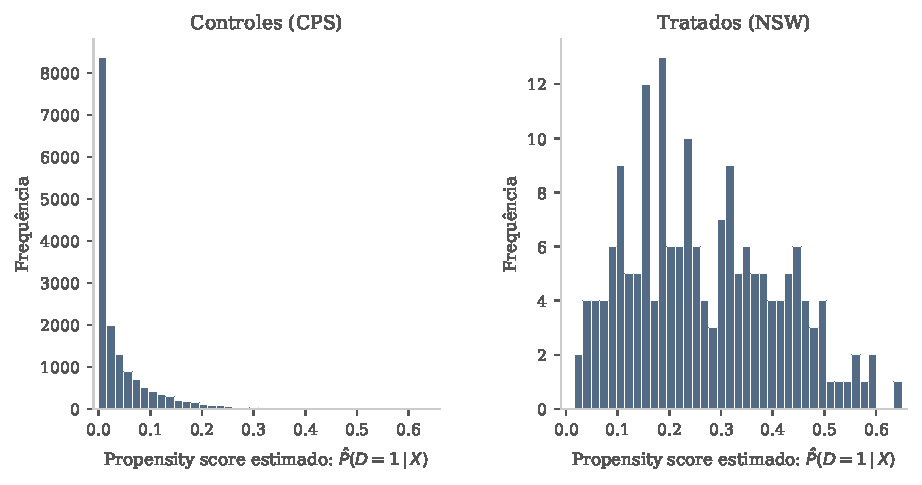
\includegraphics[width=0.85\linewidth]{Figuras/propensity_score.pdf}
\caption{Distribuição dos \textit{Propensity Scores} estimados por grupo}
\label{fig:pscore_dist}
\figmeta{Cálculo dos autores com dados do CPS e NSW.}{FGV CLEAR.}{Entre os controles (CPS), a distribuição é fortemente concentrada próxima de zero; entre os tratados (NSW), os valores são mais espalhados.}
\end{figure}

A Figura~\ref{fig:pscore_dist} ilustra um problema crítico de suporte comum: entre os controles (CPS), a distribuição do \textit{propensity score} é fortemente concentrada em valores muito próximos de zero, enquanto os tratados exibem valores substancialmente maiores. Isso indica que, sem pareamento, as comparações diretas entre grupos são inválidas. A Figura~\ref{fig:overlap} apresenta a mesma informação de forma sobreposta, evidenciando a região de suporte comum.

\begin{figure}[H]
\centering
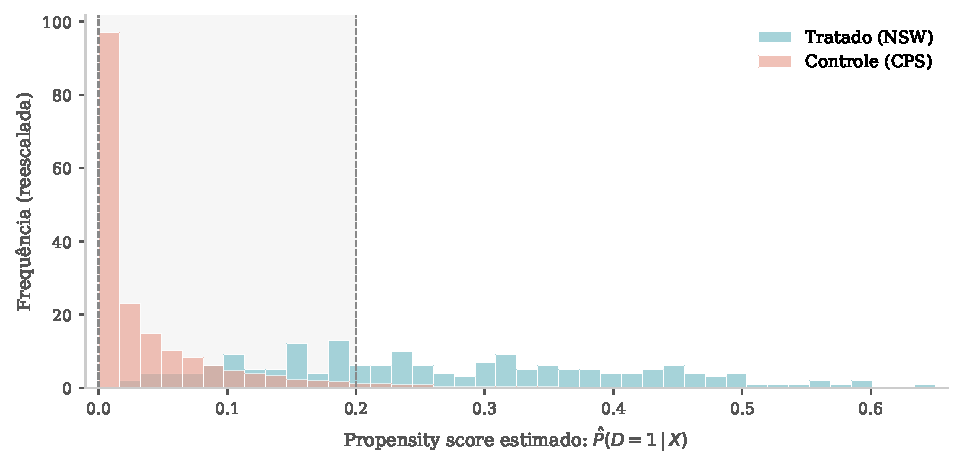
\includegraphics[width=0.75\linewidth]{Figuras/propensity_score_overlap.pdf}
\caption{Sobreposição do \textit{propensity score} por grupo}
\label{fig:overlap}
\figmeta{Cálculo dos autores com dados do CPS e NSW.}{FGV CLEAR.}{A região de sobreposição entre as distribuições delimita o suporte comum\textemdash{}apenas nesse intervalo o pareamento produz comparações válidas. As frequências dos controles (CPS) foram reescaladas proporcionalmente ao tamanho do grupo de tratados (NSW) para facilitar a comparação visual.}
\end{figure}

\subsubsection{Vizinho Mais Próximo pelo \textit{Propensity Score}}

Uma vez estimado o \textit{propensity score}, a forma mais natural de usá-lo é aplicar a lógica do vizinho mais próximo nessa única variável escalar: cada tratado é emparelhado com o(s) controle(s) cujo $\hat{p}(X_i)$ seja mais próximo ao seu.

\begin{lstlisting}[style=Rstyle]
# Preparação com propensity score
dat <- cps %>%
  dplyr::select(all_of(c("treat", "re78", covs))) %>%
  tidyr::drop_na() %>%
  mutate(treat = as.integer(treat))

ps_model <- glm(fml_ps, data = dat, family = binomial("logit"))
dat      <- dat %>% mutate(pscore = predict(ps_model, type = "response"))

Y   <- dat$re78
Tr  <- dat$treat
Xps <- as.matrix(dat$pscore)   # X unidimensional = propensity score

# Função auxiliar
run_nn_ps <- function(M, estimand = c("ATT", "ATE")) {
  estimand <- match.arg(estimand)
  out <- Match(Y = Y, Tr = Tr, X = Xps,
               M = M, replace = TRUE, estimand = estimand)
  tibble(estimand = estimand, M = M,
         estimate = out$est, se_AI = out$se)
}

# Rodar M = 1, 3, 5 (ATT e ATE)
results_ps <- bind_rows(
  lapply(c(1, 3, 5), run_nn_ps, estimand = "ATT"),
  lapply(c(1, 3, 5), run_nn_ps, estimand = "ATE")
)
\end{lstlisting}

\begin{table}[H]
\centering
\caption{Nearest Neighbor Matching pelo \textit{Propensity Score}}\label{tab:nn_ps}
\begin{tabular}{lccc}
\toprule
 & \multicolumn{3}{c}{Número de vizinhos ($M$)} \\
\cmidrule(lr){2-4}
 & $M=1$ & $M=3$ & $M=5$ \\
\midrule
\multicolumn{4}{l}{\textbf{Painel A: Efeito Médio sobre os Tratados (ATT)}} \\
\midrule
Tratamento & 1.322,142 & 1.075,699 & 1.193,554 \\
           & (943,412) & (818,544) & (812,322) \\
\midrule
\multicolumn{4}{l}{\textbf{Painel B: Efeito Médio do Tratamento (ATE)}} \\
\midrule
Tratamento & $-$4.027,222 & $-$7.149,183 & $-$7.009,720 \\
           & (4.238,945)  & (3.389,585)  & (2.771,592)  \\
\bottomrule
\multicolumn{4}{l}{\footnotesize Erros-padrão com correção analítica de Abadie--Imbens. Pareamento com reposição.}\\
\end{tabular}
\end{table}

O ATT (Painel A) é positivo e relativamente estável à escolha de $M$, sugerindo que o \textit{propensity score} consegue construir um grupo de controle mais comparável aos tratados. Em contraste, o ATE (Painel B) permanece problemático, refletindo a dificuldade de identificar efeitos causais médios em toda a população com dados não experimentais.

\subsubsection{Ponderação pelo \textit{Propensity Score} (IPW)}

Há uma segunda forma de explorar o \textit{propensity score}: em vez de selecionar vizinhos, utilizá-lo diretamente para construir pesos. Essa abordagem é conhecida como \textit{Inverse Probability Weighting} (IPW).

A lógica econômica é a seguinte: se indivíduos com diferentes probabilidades de tratamento estão desproporcionalmente representados nos grupos, podemos reponderar as observações de modo que, após a ponderação, a composição dos grupos se torne comparável. O estimador de IPW para o ATE é:
$$\widehat{\text{ATE}}_{\text{IPW}} = \frac{1}{N}\sum_{i=1}^N\left(\frac{D_i Y_i}{\hat{p}(X_i)} - \frac{(1-D_i)Y_i}{1-\hat{p}(X_i)}\right)$$

E para o ATT:
$$\widehat{\text{ATT}}_{\text{IPW}} = \frac{1}{N_1}\sum_{i:D_i=1} Y_i - \frac{1}{N_1}\sum_{i:D_i=0} \frac{\hat{p}(X_i)}{1-\hat{p}(X_i)} Y_i$$

em que $N_1$ é o número de tratados. Nesse segundo estimador, os tratados entram com peso unitário e os controles são reponderados para reproduzir a distribuição dos tratados em termos de \textit{propensity score}.

\begin{lstlisting}[style=Rstyle]
# Trimming: remover extremos do propensity score (recomendado)
dat <- dat %>%
  filter(pscore > 0.1, pscore < 0.9)

# Calcular pesos
dat <- dat %>%
  mutate(
    w_ate = treat / pscore + (1 - treat) / (1 - pscore),
    w_att = ifelse(treat == 1, 1, pscore / (1 - pscore))
  )

# Estimativas IPW
fit_ate <- lm_robust(re78 ~ treat, data = dat, weights = w_ate)
fit_att <- lm_robust(re78 ~ treat, data = dat, weights = w_att)
\end{lstlisting}

\begin{table}[H]
\centering
\caption{Estimativas por Ponderação Inversa da Probabilidade (IPW)}\label{tab:ipw}
\begin{tabular}{lcc}
\toprule
 & ATE & ATT \\
\midrule
Tratamento \hspace{50mm} & 1.533,798$^+$ & 2.056,846** \\
                          & (807,560) & (775,559) \\
Obs. & 452 & 452 \\
\bottomrule
\multicolumn{3}{l}{\footnotesize $^{+}\,p<0{,}1$;\; $^{*}\,p<0{,}05$;\; $^{**}\,p<0{,}01$;\; $^{***}\,p<0{,}001$. \textit{Trimming}: $\hat{p} \in (0{,}1;\,0{,}9)$.}\\
\end{tabular}
\end{table}

O IPW produz estimativas de ATE e ATT que se aproximam substancialmente do efeito experimental, sugerindo que a reponderação consegue reproduzir de forma mais adequada o contrafactual relevante.

\begin{notabox}[Sensibilidade a pesos extremos]
A ponderação é particularmente sensível a problemas de suporte comum. Se houver indivíduos com $\hat{p}(X_i)$ muito próximo de 0 ou de 1, os pesos $1/\hat{p}(X_i)$ tornam-se extremamente elevados, fazendo com que poucas observações dominem o estimador. Por esse motivo, é prática padrão aplicar \textit{trimming} no \textit{propensity score}, excluindo valores extremos (ex.: $\hat{p} < 0{,}1$ ou $\hat{p} > 0{,}9$) ou truncar diretamente os pesos.
\end{notabox}

\subsection{Notas sobre Inferência}

Os estimadores de pareamento dependem de objetos estimados em uma primeira etapa, o que torna inadequada a aplicação direta de fórmulas clássicas de variância.

\textbf{Vizinho mais próximo:} a inferência é particularmente delicada devido à não suavidade do estimador e à reutilização de observações com reposição. Utilizamos a correção analítica proposta por \citet{abadie2006large}, implementada diretamente pelo objeto retornado pela função \texttt{Match()}:

\begin{lstlisting}[style=Rstyle]
# Estimativa pontual e erro-padrão com correção Abadie-Imbens
out_att <- Match(Y = Y, Tr = Tr, X = Xps,
                 M = 1, replace = TRUE, estimand = "ATT")

# Estimativa
out_att$est

# Erro-padrão com correção analítica de Abadie-Imbens
out_att$se

# Intervalo de confiança de 95%
ci_lb <- out_att$est - 1.96 * out_att$se
ci_ub <- out_att$est + 1.96 * out_att$se
cat("IC 95%: [", round(ci_lb, 2), ",", round(ci_ub, 2), "]\n")
\end{lstlisting}

\textbf{Por que o bootstrap padrão falha no NN matching?} O estimador de vizinho mais próximo é \textit{não suave}: pequenas perturbações na amostra podem alterar discretamente quais pares são formados. O bootstrap reamostral trata essa descontinuidade como variabilidade adicional, inflando artificialmente os erros-padrão. A correção de Abadie--Imbens evita esse problema por derivação analítica da variância.

\textbf{IPW e estimadores duplamente robustos:} a inferência para IPW prática costuma ser realizada por erros-padrão robustos de regressões ponderadas. Esse procedimento trata o \textit{propensity score} estimado como conhecido, subestimando a variância real. O estimador duplamente robusto (AIPW) combina um modelo de seleção e um modelo de resultado, sendo consistente se ao menos um dos dois estiver corretamente especificado:

\begin{lstlisting}[style=Rstyle]
library(AIPW)
library(SuperLearner)

# Estimador duplamente robusto (AIPW)
aipw_obj <- AIPW$new(
  Y = dat$re78,
  A = dat$treat,
  W = dat[, covs],
  Q.SL.library = c("SL.glm", "SL.ranger"),
  g.SL.library  = c("SL.glm", "SL.ranger"),
  k_split = 5,
  verbose = FALSE
)
aipw_obj$fit()
aipw_obj$summary(g.bound = 0.025)
\end{lstlisting}

\textbf{Erros-padrão clusterizados:} quando as unidades de observação estão agrupadas (alunos em escolas, trabalhadores em firmas, municípios em estados), a variância dos estimadores pode ser subestimada se não houver clusterização. Para o estimador OLS pós-pareamento, erros clusterizados são diretos:

\begin{lstlisting}[style=Rstyle]
library(estimatr)

# Criar amostra pareada
dados_pareados <- rbind(
  dat[out_att$index.treated, ],
  dat[out_att$index.control, ]
)

# OLS pós-pareamento com erros clusterizados por município
fit_cluster <- lm_robust(
  re78 ~ treat,
  data    = dados_pareados,
  clusters = dados_pareados$municipio,  # variável de cluster
  se_type = "CR2"
)
summary(fit_cluster)
\end{lstlisting}

\begin{notabox}[Qual abordagem de inferência usar?]
\begin{itemize}[leftmargin=1.2em, itemsep=2pt]
  \item \textbf{Vizinho mais próximo (ATT):} correção analítica de Abadie--Imbens via \texttt{Match()}
  \item \textbf{IPW simples:} erros robustos na regressão ponderada
  \item \textbf{Máxima eficiência e robustez:} estimador AIPW com \textit{cross-fitting}
  \item \textbf{Dados agrupados:} erros clusterizados no nível do grupo (escola, firma, município)
  \item \textbf{Bootstrap:} válido apenas para IPW e \textit{kernel}; \textbf{não} para vizinho mais próximo
\end{itemize}
\end{notabox}

% ==========================================
% SEÇÃO 6: EXTENSÕES E DIAGNÓSTICOS
% ==========================================
\newpage
\section{Extensões, Diagnósticos e Armadilhas}\label{sec:diagnosticos}

\subsection{Diagnóstico: Verificação do Balanceamento}

O balanceamento das covariáveis pós-pareamento é o diagnóstico mais importante para avaliar a qualidade do procedimento. Mesmo que o pareamento seja formalmente correto, covariáveis desequilibradas após o procedimento indicam que a CIA não está sendo bem aproximada.

As medidas mais utilizadas são a \textbf{diferença padronizada} (\textit{standardized mean difference}, SMD) de cada covariável antes e depois do pareamento:
$$\text{SMD} = \frac{\bar{X}_{D=1} - \bar{X}_{D=0}}{\sqrt{(s_{D=1}^2 + s_{D=0}^2)/2}}$$

Uma regra de bolso comum é aceitar SMD $< 0{,}1$ após o pareamento. O pacote \texttt{cobalt} do R facilita essa análise por meio de gráficos \textit{love plots} (ver Figura~\ref{fig:overlap} para inspeção visual do suporte comum pré-pareamento):

\begin{lstlisting}[style=Rstyle]
library(cobalt)

# Love plot para o matching por propensity score
# (objeto 'out' gerado pelo Match() com M=1, estimand="ATT")
love.plot(out, stats = "mean.diffs",
          thresholds = c(m = 0.1),
          var.order = "unadjusted",
          title = "Balanceamento: antes e após o pareamento")
\end{lstlisting}

\subsection{Métodos Alternativos}

O pareamento baseado em distância e \textit{kernel} não esgota o espectro de métodos disponíveis. Destacam-se:

\textbf{Pareamento Exato Grosseiro} (\textit{Coarsened Exact Matching} --- CEM): discretiza as covariáveis em estratos e aplica pareamento exato nesses estratos. Combina a transparência do pareamento exato com maior cobertura da amostra \citep{IacusKingPorro2012}.

\textbf{Equilíbrio por Entropia} (\textit{Entropy Balancing}): constrói pesos que equalizam exatamente momentos pré-especificados (médias, variâncias) das covariáveis entre os grupos, sem estimar explicitamente o \textit{propensity score} \citep{Hainmueller2012}. É especialmente útil quando o modelo de seleção é difícil de especificar.

\textbf{Estimadores Duplamente Robustos} (AIPW, TMLE): combinam um modelo de seleção e um modelo de resultado (\textit{outcome model}), sendo consistentes se ao menos um dos dois modelos estiver corretamente especificado \citep{ChernozhukovEtAl2018}.

\subsection{Armadilhas Comuns}

\textbf{Armadilha 1: Balanceamento pré-tratamento mas não em tendências.} Se os grupos diferem em trajetórias pré-tratamento (não apenas em níveis), o pareamento simples pode não corrigir o viés. Combinar pareamento com Diferenças-em-Diferenças (\textit{DiD + Matching}) pode resolver esse problema.

\textbf{Armadilha 2: Suporte comum insuficiente.} Quando os grupos têm pouca sobreposição, o pareamento descarta muitas observações e o estimando estimado pode ser muito diferente do ATT na população tratada original. Sempre inspecione a distribuição do \textit{propensity score} e reporte quantas observações foram descartadas.

\textbf{Armadilha 3: Especificação do \textit{propensity score}.} Um bom ajuste preditivo do modelo de seleção não garante estimativas causais válidas. O que importa é que as covariáveis relevantes para a CIA estejam incluídas, não que o modelo tenha $R^2$ alto.

\textbf{Armadilha 4: Viés residual por variáveis não observadas.} O pareamento não é um substituto para estratégias de identificação mais fortes (instrumentos, RDD, DiD) quando há seleção em não observáveis relevantes. A análise de sensibilidade de Rosenbaum \citep{RosenbaumRubin1983sensitiv} quantifica o quão grande precisaria ser o viés por não observáveis para invalidar as conclusões. O parâmetro $\Gamma$ mede a razão máxima de chances de tratamento entre dois indivíduos idênticos nas variáveis observadas: $\Gamma = 1$ corresponde a nenhum viés não observado; $\Gamma = 2$ significa que dois indivíduos comparáveis podem diferir até duas vezes na probabilidade de tratamento por fatores não observados.

\begin{lstlisting}[style=Rstyle]
library(rbounds)

# Análise de sensibilidade de Rosenbaum
# 'out_att' é o objeto Match() com estimand="ATT"
# Extrair resultados dos pares
y_tratado  <- dat$re78[out_att$index.treated]
y_controle <- dat$re78[out_att$index.control]

# Teste de Wilcoxon com limites de sensibilidade
psens(y_tratado - y_controle,
      Gamma    = 2,     # testar até Gamma = 2
      GammaInc = 0.1)   # incremento de 0.1

# Interpretação: o menor Gamma para o qual o
# p-valor supera 0.05 é o "Gamma crítico".
# Um Gamma crítico alto indica robustez a não observáveis.
\end{lstlisting}

\begin{notabox}[Como interpretar o $\Gamma$ crítico]
Se o $\Gamma$ crítico for próximo de 1 (ex.: $\Gamma^* = 1{,}2$), a conclusão causal é frágil: um fator não observado que dobrasse levemente as chances de tratamento já invalidaria o resultado. Se $\Gamma^* > 2$, o efeito é robusto a vieses moderados por não observáveis. Reporte sempre o $\Gamma$ crítico junto com as estimativas principais.
\end{notabox}

\textbf{Armadilha 5: Erros-padrão incorretos.} Ao usar \textit{propensity score} estimado, erros-padrão de regressões ponderadas subestimam a variância real. Para inferência rigorosa, utilize a correção de Abadie--Imbens (vizinho mais próximo) ou bootstrap robusto (IPW).

\begin{table}[H]
\centering
\caption{Resumo de diagnósticos e soluções para problemas comuns no pareamento}
\label{tab:diagnosticos_resumo}
\footnotesize
\begin{tabular}{p{3.5cm}p{4cm}p{5.5cm}}
\toprule
\textbf{Problema} & \textbf{Diagnóstico} & \textbf{Solução} \\
\midrule
Balanceamento ruim pós-pare\-amento & SMD $> 0{,}1$ em covariáveis-chave & Mais vizinhos; \textit{caliper}; mudança de métrica \\
Suporte comum insuficiente & Muitas obs.\ descartadas; propensity scores extremos & \textit{Trimming}; restringir população alvo \\
Viés residual & Sensibilidade ao conjunto de covariáveis & CEM, entropia, análise de sensibilidade \\
Erros-padrão incorretos & SE subestimados & Correção A--I; bootstrap \\
Seleção em não observáveis & Resultados instáveis à especificação & Métodos complementares (DiD, IV, RDD) \\
\bottomrule
\multicolumn{3}{l}{\footnotesize \textbf{Elaboração:} FGV CLEAR.}
\end{tabular}
\end{table}

% ==========================================
% SEÇÃO 7: APLICAÇÕES
% ==========================================
\newpage
\section{Aplicações em Políticas Públicas}\label{sec:aplicacoes}

O pareamento já foi amplamente utilizado em diferentes áreas de políticas públicas como estratégia central de avaliação causal em contextos nos quais experimentos aleatorizados não são viáveis. Em muitas políticas reais, a randomização esbarra em restrições éticas, políticas ou operacionais. Nesses ambientes, avaliações baseadas exclusivamente em comparações ingênuas tendem a produzir estimativas fortemente enviesadas \citep{rosenbaum1983central,rubin1974estimating}.

\subsection*{Educação}

Na área de educação, o pareamento tem sido amplamente empregado na avaliação de programas de educação complementar, como cursos técnicos, programas de qualificação profissional, bolsas de estudo e tutorias acadêmicas. Esses programas raramente são alocados aleatoriamente: a participação costuma depender de características individuais, critérios administrativos, decisões familiares ou da própria escola, gerando forte seleção dos participantes.

Avaliações baseadas em pareamento constroem grupos de comparação a partir de indivíduos não participantes com perfil semelhante em termos de idade, escolaridade prévia, desempenho acadêmico, renda familiar, características da escola e localização geográfica, permitindo estimar efeitos causais sobre progressão educacional, evasão, desempenho em testes e inserção no mercado de trabalho \citep{heckman1997matching,smith2005does}.

\textbf{No contexto brasileiro}, o pareamento por \textit{propensity score} tem sido utilizado para avaliar o impacto do PRONATEC sobre empregabilidade e renda de jovens egressos. Utilizando dados administrativos da RAIS e do Cadastro Nacional de Informações Sociais (CNIS), avaliações combinam pareamento com diferenças-em-diferenças para comparar trabalhadores formais que frequentaram cursos do programa com trabalhadores de perfil similar que não participaram, controlando por setor de atividade, escolaridade, renda pré-programa e região. Um desafio central nessas aplicações é a qualidade dos registros de participação, que pode ser incompleta para cursos de curta duração.

Um conjunto particularmente influente de estudos comparou estimativas obtidas via pareamento com resultados de experimentos aleatorizados em programas de treinamento nos Estados Unidos, mostrando que, quando o conjunto de covariáveis é rico e o suporte comum é adequadamente respeitado, o pareamento consegue reproduzir de forma bastante próxima os efeitos experimentais \citep{dehejia1999causal,dehejia2002propensity}.

\subsection*{Saúde}

Na área da saúde, o pareamento é frequentemente utilizado para avaliar programas de prevenção, acompanhamento médico e intervenções em saúde pública. Indivíduos mais atentos à própria saúde tendem simultaneamente a participar das intervenções e a apresentar melhores desfechos, mesmo na ausência do programa. O pareamento contribui para mitigar esse viés ao construir grupos comparáveis em termos de histórico médico, utilização prévia de serviços de saúde e perfil demográfico \citep{stuart2010matching}.

\textbf{No Brasil}, avaliações do Programa Saúde da Família (PSF/ESF) utilizaram pareamento para comparar municípios com e sem cobertura pela Estratégia Saúde da Família, controlando por porte populacional, índice de desenvolvimento humano, cobertura de saneamento básico e gastos per capita em saúde. Resultados desse tipo de análise sugerem reduções nas taxas de mortalidade infantil e hospitalizações por condições sensíveis à atenção primária em municípios com maior cobertura da ESF. Nessas aplicações com dados municipais, a unidade de observação é o município, e o pareamento é realizado sobre indicadores socioeconômicos e de infraestrutura de saúde observados antes da implantação do programa.

Em aplicações baseadas em grandes bases administrativas e registros hospitalares, o pareamento desempenha um papel fundamental ao tornar esses dados observacionais utilizáveis para inferência causal \citep{imbens2015causal}.

\subsection*{Transferência de Renda e Assistência Social}

O Brasil dispõe de um dos maiores programas de transferência de renda condicionada do mundo, o Bolsa Família (hoje Bolsa Família reformulado no âmbito do Programa Auxílio Brasil/Bolsa Família). A avaliação do programa combina desafios metodológicos específicos: a elegibilidade é determinada por renda per capita familiar, gerando forte descontinuidade; a cobertura varia substancialmente entre municípios e ao longo do tempo; e os efeitos podem se manifestar em múltiplas gerações.

Avaliações baseadas em pareamento utilizam os dados do CadÚnico para comparar famílias elegíveis que participam do programa com famílias de perfil similar que ainda não foram incorporadas (listas de espera) ou que vivem em municípios com baixa cobertura. Covariáveis típicas incluem composição domiciliar, renda per capita, escolaridade do responsável, condições de moradia e acesso a serviços. Resultados encontrados na literatura brasileira incluem efeitos positivos sobre frequência escolar, redução do trabalho infantil e, em menor grau, indicadores nutricionais de crianças beneficiárias.

\subsection*{Mercado de Trabalho}

No mercado de trabalho, técnicas de pareamento ocupam um papel central na avaliação de políticas ativas de emprego, como subsídios à contratação, programas de intermediação de mão de obra, seguro-desemprego e iniciativas de qualificação profissional. Avaliações empíricas comparam beneficiários com trabalhadores de perfil semelhante em termos de idade, escolaridade, ocupação anterior, histórico de emprego, duração do desemprego e região de residência \citep{heckman1998characterizing,caliendo2008some,lechner2011matching}.

\textbf{No Brasil}, a RAIS (Relação Anual de Informações Sociais) e o CAGED (Cadastro Geral de Empregados e Desempregados) oferecem dados administrativos longitudinais de alta qualidade sobre vínculos formais de emprego, permitindo construir históricos de trabalho detalhados para matching. Avaliações do seguro-desemprego, por exemplo, utilizam pareamento para comparar trabalhadores demitidos sem justa causa que solicitaram o benefício com trabalhadores em situação similar que não o solicitaram, controlando por setor, porte da firma, salário anterior e tempo de emprego.

\subsection*{Boas Práticas}

A ampla aplicação do pareamento em políticas públicas levou ao desenvolvimento de um conjunto de boas práticas: verificação sistemática de balanceamento das covariáveis após o pareamento, análise explícita do suporte comum, avaliação da sensibilidade dos resultados a diferentes especificações, e uso de procedimentos apropriados de inferência estatística \citep{abadie2006large}.

O pareamento não cria informação onde ela não existe: quando não há sobreposição suficiente entre tratados e controles, a consequência lógica é a exclusão de observações e a redefinição do parâmetro causal estimado. Ao tornar explícitas as hipóteses identificadoras e as limitações impostas pelos dados, o método contribui para avaliações mais transparentes e replicáveis.

\begin{tcolorbox}[colback=orangebg, colframe=orangeframe, boxrule=0.5pt, arc=2pt,
  left=6pt, right=6pt, top=4pt, bottom=4pt]
\textcolor{orangeframe}{\textbf{Bases de dados brasileiras frequentemente usadas com pareamento:}}
\textit{RAIS/CAGED} (mercado de trabalho formal); \textit{CadÚnico} (programas sociais); \textit{SINASC/SIM} (saúde materno-infantil); \textit{SAEB/Prova Brasil} (educação); \textit{IBGE-PNAD Contínua} (condições de vida); \textit{DataSUS/SIH} (internações hospitalares). Bases administrativas longitudinais permitem construir covariáveis pré-tratamento ricas, favorecendo a plausibilidade da CIA.
\end{tcolorbox}

% ==========================================
% FICHA RÁPIDA
% ==========================================
\newpage
\section*{Ficha Rápida: Checklist de Implementação}
\addcontentsline{toc}{section}{Ficha Rápida: Checklist de Implementação}

\noindent Use esta ficha como referência rápida ao aplicar o pareamento em uma avaliação real. Cada etapa remete à seção correspondente do guia.

\vspace{0.4cm}

\begin{tcolorbox}[colback=salmonbg, colframe=salmonframe, boxrule=0.5pt, arc=2pt,
  title={\bfseries Etapa 1 — Definir o estimando e verificar a CIA (Seções 2--3)},
  coltitle=black, fonttitle=\bfseries, left=6pt, right=6pt]
\begin{itemize}[leftmargin=1.2em, itemsep=2pt]
  \item[$\square$] Definir claramente se o parâmetro de interesse é o ATT ou o ATE
  \item[$\square$] Listar as variáveis que determinam a seleção no tratamento (consulte um DAG)
  \item[$\square$] Garantir que nenhuma covariável na lista seja pós-tratamento ou \textit{collider}
  \item[$\square$] Verificar disponibilidade de dados para todas as covariáveis relevantes antes de iniciar
\end{itemize}
\end{tcolorbox}

\vspace{0.3cm}

\begin{tcolorbox}[colback=bluebg, colframe=blueframe, boxrule=0.5pt, arc=2pt,
  title={\bfseries Etapa 2 — Verificar o suporte comum (Seção 5.2.1)},
  coltitle=white, fonttitle=\bfseries, left=6pt, right=6pt]
\begin{itemize}[leftmargin=1.2em, itemsep=2pt]
  \item[$\square$] Estimar o \textit{propensity score} e plotar a distribuição por grupo
  \item[$\square$] Inspecionar a sobreposição: há tratados sem controles comparáveis?
  \item[$\square$] Reportar quantas observações são descartadas por falta de suporte comum
  \item[$\square$] Se sobreposição for muito limitada, reconsiderar o estimando ou a amostra
\end{itemize}
\end{tcolorbox}

\vspace{0.3cm}

\begin{tcolorbox}[colback=salmonbg, colframe=salmonframe, boxrule=0.5pt, arc=2pt,
  title={\bfseries Etapa 3 — Executar o pareamento (Seções 4--5)},
  coltitle=black, fonttitle=\bfseries, left=6pt, right=6pt]
\begin{itemize}[leftmargin=1.2em, itemsep=2pt]
  \item[$\square$] Escolher o método (vizinho mais próximo, \textit{kernel}, Mahalanobis, IPW)
  \item[$\square$] Definir o número de vizinhos $M$ e testar sensibilidade a essa escolha
  \item[$\square$] Aplicar \textit{caliper} se necessário para evitar pareamentos distantes
  \item[$\square$] Para IPW: aplicar \textit{trimming} em propensity scores extremos ($\hat{p} < 0{,}05$ ou $> 0{,}95$)
\end{itemize}
\end{tcolorbox}

\vspace{0.3cm}

\begin{tcolorbox}[colback=bluebg, colframe=blueframe, boxrule=0.5pt, arc=2pt,
  title={\bfseries Etapa 4 — Verificar o balanceamento (Seção 6.1)},
  coltitle=white, fonttitle=\bfseries, left=6pt, right=6pt]
\begin{itemize}[leftmargin=1.2em, itemsep=2pt]
  \item[$\square$] Calcular SMD antes e depois do pareamento para cada covariável
  \item[$\square$] Critério: SMD $< 0{,}1$ após pareamento para todas as covariáveis relevantes
  \item[$\square$] Gerar \textit{love plot} com o pacote \texttt{cobalt} e incluir no relatório
  \item[$\square$] Se balanceamento ruim: tentar mais vizinhos, método diferente ou respecificar propensity score
\end{itemize}
\end{tcolorbox}

\vspace{0.3cm}

\begin{tcolorbox}[colback=salmonbg, colframe=salmonframe, boxrule=0.5pt, arc=2pt,
  title={\bfseries Etapa 5 — Inferência e análise de sensibilidade (Seções 5.4 e 6.3)},
  coltitle=black, fonttitle=\bfseries, left=6pt, right=6pt]
\begin{itemize}[leftmargin=1.2em, itemsep=2pt]
  \item[$\square$] Vizinho mais próximo: usar correção analítica de Abadie--Imbens (\texttt{Matching::Match})
  \item[$\square$] IPW: usar erros-padrão robustos ou estimador duplamente robusto (AIPW)
  \item[$\square$] Executar análise de sensibilidade de Rosenbaum (\texttt{rbounds}) e reportar $\Gamma$ crítico
  \item[$\square$] Verificar estabilidade das estimativas a diferentes especificações do modelo de seleção
\end{itemize}
\end{tcolorbox}

\vspace{0.3cm}

\begin{tcolorbox}[colback=orangebg, colframe=orangeframe, boxrule=0.5pt, arc=2pt,
  left=6pt, right=6pt, top=4pt, bottom=4pt]
\textcolor{orangeframe}{\textbf{Quando NÃO usar apenas o pareamento:}} se houver razões para crer que a seleção depende de variáveis não observadas (motivação, expectativas, informação privada), o pareamento por si só não identifica o efeito causal. Considere combiná-lo com DiD, ou migrar para uma estratégia de identificação mais forte (IV, RDD).
\end{tcolorbox}

% ==========================================
% SEÇÃO 8: CONCLUSÃO
% ==========================================
\newpage
\section{Conclusão}\label{sec:conclusao}

Este guia apresentou de forma sistemática os fundamentos conceituais e operacionais do pareamento, posicionando-o dentro do arcabouço geral de inferência causal da série \textit{Avaliação na Prática}. Assim como no caso de estratégias experimentais e quase-experimentais, o objetivo central permanece o mesmo: recuperar um contrafactual plausível que permita estimar efeitos causais com rigor e transparência.

O pareamento oferece uma resposta particularmente útil para contextos em que a aleatorização não é possível e em que a construção de um grupo de controle comparável depende das características observáveis. Ao aproximar a distribuição dessas covariáveis entre tratados e controles, minimizamos o viés de seleção decorrente da alocação não aleatória do tratamento.

As principais mensagens são:

\begin{enumerate}[leftmargin=1.5cm]
  \item A validade do pareamento repousa sobre a Hipótese de Independência Condicional --- que a seleção no tratamento seja explicada inteiramente pelas covariáveis observadas;
  \item O \textit{propensity score} resolve o problema da maldição da dimensionalidade ao resumir todas as covariáveis em uma única variável escalar, mas não substitui a CIA;
  \item A verificação do balanceamento pós-pareamento é tão importante quanto a estimação do efeito: um SMD $< 0{,}1$ é condição necessária para interpretar os resultados causalmente;
  \item Quando há tendências pré-tratamento diferentes entre grupos, combinar pareamento com Diferenças-em-Diferenças pode ser mais adequado;
  \item A inferência rigorosa requer a correção de Abadie--Imbens para vizinho mais próximo e técnicas de bootstrap ou estimadores duplamente robustos para IPW.
\end{enumerate}

O pareamento não é um substituto para métodos baseados em hipóteses mais fortes (DiD, RDD, variáveis instrumentais) quando há seleção em não observáveis relevantes. É, no entanto, uma ferramenta poderosa e intuitiva para aprimorar comparações em dados observacionais, servindo tanto como estimador principal quanto como componente de estratégias híbridas.

\begin{conexaobox}
\textcolor{orangeframe}{\textbf{$\hookrightarrow$ Conexão com outros guias:}} \textit{Guia de DiD --- O DiD combina a lógica do pareamento com a comparação de tendências temporais; Matching + DiD é uma estratégia híbrida comum. Guia de Avaliação de Impacto --- apresenta o arcabouço geral de avaliação e discute quando o pareamento é adequado em relação a outros estimadores. Guia de Análise de Poder Estatístico --- o dimensionamento amostral deve levar em conta as perdas de observações decorrentes da imposição do suporte comum.}
\end{conexaobox}

% ==========================================
% REFERÊNCIAS
% ==========================================
\newpage
\bibliographystyle{apalike}

\begin{thebibliography}{99}

\bibitem[Abadie e Imbens(2006)]{abadie2006large}
Abadie, A. e Imbens, G.~W. (2006).
\newblock Large Sample Properties of Matching Estimators for Average Treatment Effects.
\newblock \textit{Econometrica}, 74(1), 235--267.

\bibitem[Abadie e Imbens(2011)]{AbadiImbens2011}
Abadie, A. e Imbens, G.~W. (2011).
\newblock Bias-Corrected Matching Estimators for Average Treatment Effects.
\newblock \textit{Journal of Business \& Economic Statistics}, 29(1), 1--11.

\bibitem[Caliendo e Kopeinig(2008)]{caliendo2008some}
Caliendo, M. e Kopeinig, S. (2008).
\newblock Some Practical Guidance for the Implementation of Propensity Score Matching.
\newblock \textit{Journal of Economic Surveys}, 22(1), 31--72.

\bibitem[Chernozhukov et al.(2018)]{ChernozhukovEtAl2018}
Chernozhukov, V., Chetverikov, D., Demirer, M., Duflo, E., Hansen, C., Newey, W.\ e Robins, J. (2018).
\newblock Double/Debiased Machine Learning for Treatment and Structural Parameters.
\newblock \textit{The Econometrics Journal}, 21(1), C1--C68.

\bibitem[Dehejia e Wahba(1999)]{dehejia1999causal}
Dehejia, R.~H. e Wahba, S. (1999).
\newblock Causal Effects in Nonexperimental Studies: Reevaluating the Evaluation of Training Programs.
\newblock \textit{Journal of the American Statistical Association}, 94(448), 1053--1062.

\bibitem[Dehejia e Wahba(2002)]{dehejia2002propensity}
Dehejia, R.~H. e Wahba, S. (2002).
\newblock Propensity Score-Matching Methods for Nonexperimental Causal Studies.
\newblock \textit{Review of Economics and Statistics}, 84(1), 151--161.

\bibitem[Hainmueller(2012)]{Hainmueller2012}
Hainmueller, J. (2012).
\newblock Entropy Balancing for Causal Effects.
\newblock \textit{Political Analysis}, 20(1), 25--46.

\bibitem[Heckman, Ichimura e Todd(1997)]{heckman1997matching}
Heckman, J., Ichimura, H. e Todd, P. (1997).
\newblock Matching as an Econometric Evaluation Estimator.
\newblock \textit{Review of Economic Studies}, 65(2), 261--294.

\bibitem[Heckman, LaLonde e Smith(1998)]{heckman1998characterizing}
Heckman, J., LaLonde, R. e Smith, J. (1998).
\newblock The Economics and Econometrics of Active Labor Market Programs.
\newblock In O.\ Ashenfelter e D.\ Card (eds.), \textit{Handbook of Labor Economics}, vol.~3A.
\newblock Elsevier.

\bibitem[Iacus, King e Porro(2012)]{IacusKingPorro2012}
Iacus, S.~M., King, G. e Porro, G. (2012).
\newblock Causal Inference without Balance Checking: Coarsened Exact Matching.
\newblock \textit{Political Analysis}, 20(1), 1--24.

\bibitem[Imbens(2004)]{imbens2004nonparametric}
Imbens, G.~W. (2004).
\newblock Nonparametric Estimation of Average Treatment Effects Under Exogeneity: A Review.
\newblock \textit{Review of Economics and Statistics}, 86(1), 4--29.

\bibitem[Imbens e Rubin(2015)]{ImbensRubin2015}
Imbens, G.~W. e Rubin, D.~B. (2015).
\newblock \textit{Causal Inference for Statistics, Social, and Biomedical Sciences}.
\newblock Cambridge University Press.

\bibitem[Imbens e Wooldridge(2009)]{imbens2015causal}
Imbens, G.~W. e Wooldridge, J.~M. (2009).
\newblock Recent Developments in the Econometrics of Program Evaluation.
\newblock \textit{Journal of Economic Literature}, 47(1), 5--86.

\bibitem[LaLonde(1986)]{LalondeNSW1986}
LaLonde, R.~J. (1986).
\newblock Evaluating the Econometric Evaluations of Training Programs with Experimental Data.
\newblock \textit{American Economic Review}, 76(4), 604--620.

\bibitem[Lechner(2011)]{lechner2011matching}
Lechner, M. (2011).
\newblock The Estimation of Causal Effects by Difference-in-Difference Methods.
\newblock \textit{Foundations and Trends in Econometrics}, 4(3), 165--224.

\bibitem[Lin(2013)]{LinRegression2013}
Lin, W. (2013).
\newblock Agnostic Notes on Regression Adjustments to Experimental Data.
\newblock \textit{Annals of Applied Statistics}, 7(1), 295--318.

\bibitem[Rosenbaum e Rubin(1983)]{RosenbaumRubin1983}
Rosenbaum, P.~R. e Rubin, D.~B. (1983).
\newblock The Central Role of the Propensity Score in Observational Studies for Causal Effects.
\newblock \textit{Biometrika}, 70(1), 41--55.

\bibitem[Rosenbaum(1987)]{RosenbaumRubin1983sensitiv}
Rosenbaum, P.~R. (1987).
\newblock Sensitivity Analysis for Certain Permutation Inferences in Matched Observational Studies.
\newblock \textit{Biometrika}, 74(1), 13--26.

\bibitem[Rosenbaum(1987b)]{rosenbaum1983central}
Rosenbaum, P.~R. (1987).
\newblock The Role of a Second Control Group in an Observational Study.
\newblock \textit{Statistical Science}, 2(3), 292--306.

\bibitem[Rubin(1974)]{rubin1974estimating}
Rubin, D.~B. (1974).
\newblock Estimating Causal Effects of Treatments in Randomized and Nonrandomized Studies.
\newblock \textit{Journal of Educational Psychology}, 66(5), 688--701.

\bibitem[Smith e Todd(2005)]{smith2005does}
Smith, J.~A. e Todd, P.~E. (2005).
\newblock Does Matching Overcome LaLonde's Critique of Nonexperimental Estimators?
\newblock \textit{Journal of Econometrics}, 125(1--2), 305--353.

\bibitem[Stuart(2010)]{stuart2010matching}
Stuart, E.~A. (2010).
\newblock Matching Methods for Causal Inference: A Review and a Look Forward.
\newblock \textit{Statistical Science}, 25(1), 1--21.

\end{thebibliography}

\end{document}